\ECSwitch
\ECHead{Electronic Companion: Complete Proofs, Lean~4 Audit Map, and Extended Benchmarks}

\section{Complete Mathematical Proofs}\label{ec:proofs}

\subsection{Proof of Proposition~\ref*{prop:subspace} (Self-Normalized Clipping Bias and Parseval Separation)}

\proof{Proof of Proposition~\ref*{prop:subspace}.}
\emph{Part 1.} For $\pi_{\mathrm{occ}}(\psi) > 0$ and $\rho(\psi) = \frac{\mathrm{d}\nu}{\mathrm{d}\pi_{\mathrm{occ}}}(\psi) \ge 0$, pointwise inspection gives $\rho(\psi) - \min\{\bar{w}, \rho(\psi)\} = \max\{0, \rho(\psi) - \bar{w}\} \ge 0$ (\texttt{debiased\_measure\_deficit\_eq} in \texttt{SCOLHKG/V2OR/DebiasedSubspace.lean}). Applying the triangle inequality to $\langle f, h \rangle_{\nu_{\bar{w}}} - \langle f, h \rangle_\nu = \int_{\mathcal{M}_\psi} (\min\{\bar{w}, \rho(\psi)\} - \rho(\psi)) f(\psi)h(\psi) \pi_{\mathrm{occ}}(\mathrm{d}\psi)$ yields the unnormalized bound (\texttt{debiased\_inner\_clipping\_bias\_le}). Next, let $\Delta_{\bar{w}} \coloneqq \int_{\mathcal{M}_\psi} \max\{0, \rho(\psi) - \bar{w}\}\pi_{\mathrm{occ}}(\mathrm{d}\psi)$. Because $\nu(\mathcal{M}_\psi) = 1$, integrating the pointwise deficit identity yields $1 - Z_{\bar{w}} = \Delta_{\bar{w}} \ge 0$. When $|f(\psi)h(\psi)| \le B$ almost everywhere and $Z_{\bar{w}} > 0$, $|\langle f, h \rangle_{\nu_{\bar{w}}}| \le \int_{\mathcal{M}_\psi} B\,\nu_{\bar{w}}(\mathrm{d}\psi) = Z_{\bar{w}} B$. Writing $\langle f, h \rangle_{\tilde{\nu}_{\bar{w}}} = \langle f, h \rangle_{\nu_{\bar{w}}} / Z_{\bar{w}}$, the denominator $Z_{\bar{w}}$ cancels identically:
\[
  \big|\langle f, h \rangle_{\tilde{\nu}_{\bar{w}}} - \langle f, h \rangle_{\nu_{\bar{w}}}\big|
  = \frac{1 - Z_{\bar{w}}}{Z_{\bar{w}}}\big|\langle f, h \rangle_{\nu_{\bar{w}}}\big|
  \le \frac{\Delta_{\bar{w}}}{Z_{\bar{w}}}(Z_{\bar{w}} B) = B\Delta_{\bar{w}}.
\]
Combining this bound with $|\langle f, h \rangle_{\nu_{\bar{w}}} - \langle f, h \rangle_\nu| \le B\Delta_{\bar{w}}$ via the triangle inequality yields~\eqref{eq:norm_clip_bias} (\texttt{normalized\_debiased\_inner\_clipping\_bias\_le}), vanishing whenever $\sup_\psi \rho(\psi) \le \bar{w}$.

\emph{Part 2.} Expanding $h - \theta_0$ in the $\tilde{\nu}_{\bar{w}}$-orthogonal direct sum $\operatorname{span}(\tilde{\varphi}_{S_{\mathrm{act}}}) \oplus \operatorname{span}(\tilde{\varphi}_{S_{\mathrm{act}}^c}) \oplus \{r_{\mathrm{hf}}\}$ establishes Parseval separation (\texttt{active\_pruned\_orthogonal\_decomposition}).
\Halmos\endproof

\subsection{Proof of Theorem~\ref*{thm:transfer_boundary} (Within-Policy Shift Invariance and Transfer Boundary)}

\proof{Proof of Theorem~\ref*{thm:transfer_boundary}.}
\emph{Part 1.} Since $\E[\varepsilon_\ell]=0$ and $\E[\varepsilon_\ell^2]=v_t(x)$, $\E[(\Delta_g(x)+\varepsilon_\ell)^2] = \Delta_g(x)^2 + v_t(x)$. Subtracting $\bar{Y}_{t,g}(x) = \mu_{0,g}(x) + \Delta_g(x) + \bar{\varepsilon}$ gives $Y_{t,g,\ell}(x) - \bar{Y}_{t,g}(x) = \varepsilon_\ell - \bar{\varepsilon}$ identically on every sample path (\texttt{within\_policy\_ssq\_shift\_invariant}), so $\E[S_{t,g}^2(x)/(r-1)] = v_t(x)$ for any fixed $r \ge 2$. Under outcome-dependent stopping, pooled sample variance can be biased: for i.i.d.\ Rademacher draws $\{-1, +1\}$ ($v_t = 1$), stopping at $r=2$ when the first two draws agree (probability $1/2$, $s^2 = 0$) and taking two more draws when they disagree (probability $1/2$, yielding $3$-to-$1$ counts with $s^2 = 1$ with probability $1/2$ and $2$-to-$2$ counts with $s^2 = 4/3$ with probability $1/2$) gives $\E[\hat{s}_{\mathrm{pool}}^2] = \tfrac{1}{2}[0] + \tfrac{1}{4}(1) + \tfrac{1}{4}(\tfrac{4}{3}) = \tfrac{7}{12} < 1$.

\emph{Part 2.} Substituting $\theta_t - \hat{\mu}_0 = (\Delta_{\mathrm{shift}} - b_{\mathrm{occ}}) - \xi_{\mathrm{meta}}$ and using $\E[\xi_{\mathrm{meta}}] = 0$, $\E[\xi_{\mathrm{meta}}^2] = \sigma_{\mathrm{src}}^2 / M_{\mathrm{src}}$ yields $\E[\Delta_{\mathrm{eff}}^2] = (\Delta_{\mathrm{shift}} - b_{\mathrm{occ}})^2 + \sigma_{\mathrm{src}}^2 / M_{\mathrm{src}}$ (\texttt{effective\_mismatch\_second\_moment\_with\_finite\_sources}).

\emph{Part 3.} For $\kappa_0 > 0$ and $\rho_n > 0$, $(\kappa_0 + \rho_n)^2 > 0$ and exact algebraic factoring gives
\[
  \frac{1}{\rho_n} - \frac{\kappa_0^2\Delta_{\mathrm{eff}}^2 + \rho_n}{(\kappa_0 + \rho_n)^2}
  = \frac{\kappa_0^2\big(1 + 2\rho_n/\kappa_0 - \rho_n\Delta_{\mathrm{eff}}^2\big)}{\rho_n(\kappa_0 + \rho_n)^2} > 0
  \;\Longleftrightarrow\;
  \Delta_{\mathrm{eff}}^2 < \frac{1}{\rho_n} + \frac{2}{\kappa_0},
\]
checked in Lean as \texttt{transfer\_dominates\_target\_only\_iff}.
\Halmos\endproof

\subsection{Proof of Theorem~\ref*{thm:sure_uniform} (Reference Linear \texttt{SURE} Excess-Risk Bound)}

\proof{Proof of Theorem~\ref*{thm:sure_uniform}.}
\emph{Part 1.} Set $u = 1 - \lambda$. For each coordinate $k \in \mathcal{I}$ with $\tilde{R}_k = \delta_k + \xi_k$, expanding $(u \delta_k - (1 - u)\xi_k)^2 - \xi_k^2 - \frac{3}{2}[(u^2(\delta_k + \xi_k)^2 + (1 - 2u)\sigma_k^2) - \sigma_k^2]$ yields the exact identity $-\frac{1}{2}u^2 \delta_k^2 - u(2 + u)\delta_k\xi_k - (2u + \frac{1}{2}u^2)\xi_k^2 + 3u\sigma_k^2$. Averaging over $k \in \mathcal{I}$ ($m_{\mathrm{id}} = |\mathcal{I}| > 0$) gives~\eqref{eq:sure_identity} (\texttt{sure\_excess\_loss\_minus\_three\_halves\_empirical\_gap}).

\emph{Part 2.} Since $\hat{\lambda} \in [0, 1]$, $\hat{u} = 1 - \hat{\lambda} \in [0, 1]$ and $\widehat{R}_{\mathcal{I}}(\hat{\lambda}) \le \widehat{R}_{\mathcal{I}}(1)$ implies $\frac{3}{2}(\widehat{R}_{\mathcal{I}}(\hat{\lambda}) - \widehat{R}_{\mathcal{I}}(1)) \le 0$. Dropping the non-positive noise square $-(2\hat{u} + \frac{1}{2}\hat{u}^2)\frac{1}{m_{\mathrm{id}}}\sum_{k \in \mathcal{I}}\xi_k^2 \le 0$ and using $3\hat{u}\bar{\sigma}^2 \le 3\bar{\sigma}^2$ proves the $\bar{\delta}^2 = 0$ bound (\texttt{sure\_selector\_zero\_shift\_excess\_loss\_bound}). When $\bar{\delta}^2 > 0$, $0 \le 2 + \hat{u} \le 3$ gives $-\hat{u}(2 + \hat{u})\bar{C} \le 3\hat{u}|\bar{C}|$; completing the square yields $-\frac{1}{2}\hat{u}^2 \bar{\delta}^2 + 3\hat{u}|\bar{C}| = \frac{9\bar{C}^2}{2\bar{\delta}^2} - \frac{(\hat{u}\bar{\delta}^2 - 3|\bar{C}|)^2}{2\bar{\delta}^2} \le \frac{9\bar{C}^2}{2\bar{\delta}^2}$ (\texttt{sure\_selector\_uniform\_shift\_excess\_loss\_bound}), specializing at unit proxy $\sigma_k^2 \equiv 1$ to $3 + 9\bar{C}^2/(2\bar{\delta}^2)$ (\texttt{fisher\_whitened\_unit\_variance\_sure\_bound}). In the fixed-design, known-precision reference model where $X_{n,c}^\top W_{n,c}\mathbf{1} = 0$ and true sample-mean error covariance satisfies $V_{n,c} = W_{n,c}^{-1}$, $\operatorname{Cov}(X_{n,c}^\top W_{n,c}(y_{n,c} - \bar{y}_{n,c}\mathbf{1})) = X_{n,c}^\top (W_{n,c} - \frac{W_{n,c}\mathbf{1}\mathbf{1}^\top W_{n,c}}{\mathbf{1}^\top W_{n,c}\mathbf{1}}) V_{n,c} (W_{n,c} - \frac{W_{n,c}\mathbf{1}\mathbf{1}^\top W_{n,c}}{\mathbf{1}^\top W_{n,c}\mathbf{1}}) X_{n,c} = X_{n,c}^\top W_{n,c} X_{n,c} = G_{n,c}$, so $\operatorname{Cov}(\tilde{\bm{\xi}}_{n,c}) = I_{m_{\mathrm{id}}}$. Because the online implementation plugs in adaptive HVD variance estimates $\hat{W}_{n,c} \neq V_{n,c}^{-1}$ on sequentially selected policies, its projected covariance is no longer guaranteed to equal the identity matrix $I_{m_{\mathrm{id}}}$ used in this reference calculation.

\emph{Part 3.} Under pairwise orthogonality with $\E[\xi_k^2] \le \sigma_{\max}^2$, $\E[(\sum_{k \in \mathcal{I}} \delta_k\xi_k)^2] = \sum_{k \in \mathcal{I}} \delta_k^2 \E[\xi_k^2] \le m_{\mathrm{id}}\sigma_{\max}^2 \bar{\delta}^2$, hence $\E[9\bar{C}^2/(2\bar{\delta}^2)] \le 9\sigma_{\max}^2/(2 m_{\mathrm{id}})$ (\texttt{expected\_unit\_projection\_noise\_le\_sigma\_div\_rank}).
\Halmos\endproof

\subsection{Proof of Theorem~\ref*{thm:eckg_dual_voi} and Sufficient Query-Ranking Margin}\label{ec:kg_correction}\label{ec:cascade_rank}

\proof{Proof of Theorem~\ref*{thm:eckg_dual_voi}.}
\emph{Parts 1--2.} For each fantasy node $s \in \{1,\dots,S_{\mathrm{out}}\}$ with $w_s \ge 0$, write $M_0^{(s)} = \max_{\mathcal{S} \in \mathfrak{M}_0^{(s)}} U_{n+1}(\mathcal{S})$ and $M_1^{(s)}(q) = \max_{\mathcal{S} \in \mathfrak{M}_1^{(s)}(q)} U_{n+1}(\mathcal{S})$. Because $\mathcal{S}_n^\star \in \mathfrak{M}_0^{(s)} \subseteq \mathfrak{M}_1^{(s)}(q)$, pointwise monotonicity gives $U_{n+1}(\mathcal{S}_n^\star) \le M_0^{(s)} \le M_1^{(s)}(q)$, and telescoping $(M_1^{(s)}(q) - U_{n+1}(\mathcal{S}_n^\star)) = (M_0^{(s)} - U_{n+1}(\mathcal{S}_n^\star)) + (M_1^{(s)}(q) - M_0^{(s)})$ establishes $\widehat{\mathrm{VOI}}_n^{\mathrm{EC}}(q) = \widehat{\mathrm{VOI}}_n^{\mathrm{refine}}(q) + \widehat{\mathrm{VOI}}_n^{\mathrm{admit}}(q)$ alongside non-negativity of all three quantities (\texttt{eligible\_cascade\_dual\_voi\_decomposition} and \texttt{eligible\_cascade\_components\_nonneg}). Whenever $q \in \mathcal{D}_n$, $\mathcal{D}_n \cup \{q\} = \mathcal{D}_n$ implies $\hat{\mathcal{S}}_{n+1}(\mathcal{D}_n \cup \{q\}) = \hat{\mathcal{S}}_{n+1}(\mathcal{D}_n) \in \mathfrak{M}_0^{(s)}$, so $M_1^{(s)}(q) = M_0^{(s)}$ and $\widehat{\mathrm{VOI}}_n^{\mathrm{admit}}(q) = 0$ identically (\texttt{revisit\_query\_zero\_admit\_voi}).

\emph{Part 3 and Tower-Aligned Single-Slot Quadrature.} Convexity of $z \mapsto (\hat{J}_n^{\mathrm{ref}} - z)_+$ and $\E_{\Omega_f}[\mu_{n+1,f}(x')] = \mu_{n,f}(x')$ give $\E_{\Omega_f}[(\hat{J}_n^{\mathrm{ref}} - \mu_{n+1,f}(x'))_+] \ge (\hat{J}_n^{\mathrm{ref}} - \mu_{n,f}(x'))_+$ (\texttt{hinge\_submartingale\_step}); multiplying by $\E_{\Omega_g}[p_{n+1,0}^{\mathrm{gate}}(x')] = p_{n,0}^{\mathrm{gate}}(x') \ge 0$ on $\Omega_f \times \Omega_g$ yields $\E_n[V_{n+1}(x')] \ge V_n(x')$ (\texttt{factored\_gate\_utility\_submartingale}) and non-negativity of single-slot KG (\texttt{bgp\_kg\_nonneg\_from\_posterior\_tower}). In numerical implementation, because current gate power uses a $9$-node rule $p$ while conditional fantasy power uses a $7$-node inner rule $q_j \in [0,1]$ with mean $m = \sum_j w_j q_j$, the monotone affine map $\tilde{p}_j = (p/m)q_j$ ($m > p$) and $\tilde{p}_j = 1 - [(1-p)/(1-m)](1-q_j)$ ($m < p$) preserves $[0,1]$ bounds and enforces $\sum_j w_j \tilde{p}_j = p$ identically, yielding exact zero value at zero innovation. Bounded innovations $|\Delta\mu_f| \le \varepsilon_f$, $|\Delta p_0^{\mathrm{gate}}| \le \varepsilon_g$ imply $V_{n+1}(x') \le V_n(x') + \varepsilon_f + B_f\varepsilon_g$ (\texttt{bgp\_kg\_lipschitz\_in\_step\_innovations}), which yields the conditional single-step visit bound (\texttt{greedy\_bgp\_kg\_cannot\_starve\_informative\_arm}: whenever an arm with acquisition value at least $\gamma$ exists and every arm with at least $M_{\mathrm{cap}}$ visits has acquisition value strictly below $\gamma$, the greedy rule selects an arm with fewer than $M_{\mathrm{cap}}$ visits).
\Halmos\endproof

\begin{proposition}[Sufficient Margin for Single-Slot vs.\ Cascade Query Agreement]\label{prop:cascade_rank}
Let $M_C(\mathcal{F}_{n,q}^+)$ and $M_S(\mathcal{F}_{n,q}^+)$ denote post-query full-cascade and single-slot payoffs on coupled fantasy draws, with $\E_n[|M_C(\mathcal{F}_{n,q}^+) - M_S(\mathcal{F}_{n,q}^+)|] \le e_n(q)$. Writing $G_C(q)$ and $G_S(q)$ for their increments over current baselines, a single-slot maximizer $q_\star$ is also preferred by the full cascade over every rival $q$ satisfying $G_S(q_\star) - G_S(q) > e_n(q_\star) + e_n(q)$, where $e_n(q)$ is bounded by the probabilities and cost gaps of the disjoint guard-override event $A_0 \cap A_1 \cap B^c$ and fallback rescue events $A_0^c \cap A_1$ and $A_0^c \cap A_1^c \cap A_2$.
\end{proposition}

\subsection{Proof of Theorem~\ref*{thm:vkg_safety} (Distribution-Free Clean-Up Safety)}

\proof{Proof of Theorem~\ref*{thm:vkg_safety}.}
Fix any shortlist $\mathcal{S} = (x_{(0)}, \dots, x_{(L-1)})$ conditional on $\mathcal{F}_N$. For any unsafe slot $i$ with $p_i = p_t^{\mathrm{ver}}(x_{(i)}) > \alpha$, coupling Bernoulli($p_i$) and Bernoulli($\alpha$) indicators via common uniforms shows $\Prob_{\mathbb{Q}_t^{\mathrm{ver}}}(A_i \mid \mathcal{F}_N) = \operatorname{BinomCDF}(k_i^\star; K_i, p_i) \le \operatorname{BinomCDF}(k_i^\star; K_i, \alpha) \le \delta_i$ (\texttt{binomial\_one\_violation\_gate\_power\_bound}). Under both the guarded branch and the sequential first-pass branch, every certified deployment $\hat{x}_t = x_{(i)}$ requires $A_i$ to occur on slot $i$'s fresh verification block (\texttt{v2\_objective\_guarded\_unsafe\_deployment\_subset}). Union-bounding over $\{i : p_i > \alpha\}$ gives $\Prob_{\mathbb{Q}_t^{\mathrm{ver}}}(C \cap \{p_t^{\mathrm{ver}}(\hat{x}_t) > \alpha\} \mid \mathcal{F}_N) \le \sum_{i=0}^{L-1} \delta_i \le \delta$ (\texttt{v2\_terminal\_deployment\_fwer\_le\_delta}, \texttt{v2\_terminal\_five\_percent\_asymmetric\_spend}), with total verification calls bounded by $112 + 128 + 140 = \MaxVerifCalls$ (\texttt{v2\_terminal\_calls\_le\_cap}).
\Halmos\endproof

\section{Lean~4.31.0 Mechanized Proof Map and Artifact Provenance}\label{ec:lean_map}\label{ec:provenance}

All mechanized declarations in \texttt{SCOLHKG.V2ORProofInterface} were verified under Lean~4.31.0 (commit \texttt{68218e876d2a}, Mathlib \texttt{v4.31.0}) with zero \texttt{sorry} statements; \texttt{\#print axioms} confirms that all eighteen audited core theorems depend solely on standard classical foundations \texttt{[propext, Classical.choice, Quot.sound]} (receipt \texttt{v2\_or\_eckg\_lean\_receipt.json}):
{\sloppy
\begin{itemize}
  \item \texttt{DebiasedSubspace.lean}: \texttt{debiased\_\allowbreak inner\_\allowbreak exact\_\allowbreak when\_\allowbreak bounded}, \texttt{debiased\_\allowbreak inner\_\allowbreak clipping\_\allowbreak bias\_\allowbreak le}, \texttt{normalized\_\allowbreak debiased\_\allowbreak inner\_\allowbreak clipping\_\allowbreak bias\_\allowbreak le}, \texttt{orthonormal\_\allowbreak subset\_\allowbreak parseval}, \texttt{active\_\allowbreak pruned\_\allowbreak orthogonal\_\allowbreak decomposition}, and \texttt{pruned\_\allowbreak residual\_\allowbreak pointwise\_\allowbreak square\_\allowbreak bound}.
  \item \texttt{TemperedHVD.lean} and \texttt{FunctionalTransferRisk.lean}: \texttt{within\_\allowbreak policy\_\allowbreak ssq\_\allowbreak shift\_\allowbreak invariant}, \texttt{effective\_\allowbreak mismatch\_\allowbreak second\_\allowbreak moment\_\allowbreak with\_\allowbreak finite\_\allowbreak sources}, \texttt{transfer\_\allowbreak dominates\_\allowbreak target\_\allowbreak only\_\allowbreak iff}, \texttt{binomial\_\allowbreak one\_\allowbreak violation\_\allowbreak gate\_\allowbreak power\_\allowbreak bound}, and \texttt{status\_\allowbreak quo\_\allowbreak loss\_\allowbreak roster\_\allowbreak invariant}.
  \item \texttt{SequentialTheory.lean}: \texttt{sure\_\allowbreak selector\_\allowbreak uniform\_\allowbreak shift\_\allowbreak excess\_\allowbreak loss\_\allowbreak bound}, \texttt{expected\_\allowbreak unit\_\allowbreak projection\_\allowbreak noise\_\allowbreak le\_\allowbreak sigma\_\allowbreak div\_\allowbreak rank}, \texttt{fisher\_\allowbreak whitened\_\allowbreak unit\_\allowbreak variance\_\allowbreak sure\_\allowbreak bound}, \texttt{eligible\_\allowbreak cascade\_\allowbreak dual\_\allowbreak voi\_\allowbreak decomposition}, \texttt{eligible\_\allowbreak cascade\_\allowbreak components\_\allowbreak nonneg}, \texttt{revisit\_\allowbreak query\_\allowbreak zero\_\allowbreak admit\_\allowbreak voi}, \texttt{bgp\_\allowbreak kg\_\allowbreak nonneg\_\allowbreak from\_\allowbreak posterior\_\allowbreak tower}, \texttt{bgp\_\allowbreak kg\_\allowbreak lipschitz\_\allowbreak in\_\allowbreak step\_\allowbreak innovations}, \texttt{greedy\_\allowbreak bgp\_\allowbreak kg\_\allowbreak cannot\_\allowbreak starve\_\allowbreak informative\_\allowbreak arm}, and \texttt{bellman\_\allowbreak slot0\_\allowbreak minimizes\_\allowbreak expected\_\allowbreak deployed\_\allowbreak loss}.
  \item \texttt{VerificationKGAmortization.lean}: \texttt{v2\_\allowbreak objective\_\allowbreak guarded\_\allowbreak unsafe\_\allowbreak deployment\_\allowbreak subset}, \texttt{v2\_\allowbreak terminal\_\allowbreak deployment\_\allowbreak fwer\_\allowbreak le\_\allowbreak delta}, \texttt{v2\_\allowbreak terminal\_\allowbreak five\_\allowbreak percent\_\allowbreak asymmetric\_\allowbreak spend}, \texttt{v2\_\allowbreak terminal\_\allowbreak calls\_\allowbreak le\_\allowbreak cap}, and \texttt{amortized\_\allowbreak cost\_\allowbreak le\_\allowbreak cold\_\allowbreak start\_\allowbreak iff}.
\end{itemize}
}

\paragraph{Reproducibility supplement structure.}
The review supplement provides execution snapshots for the two active ledgers ($720$ DES runs and $656$ follow-up runs), the earlier $384$-run matched study, the $432$-run single-slot study, and the $9{,}796$-run predecessor benchmark, alongside the five compact fitted source priors (\texttt{prior\_default.pkl}, $75\text{ KB}$ total) so optional diagnostic replays run self-contained without external source archives. It includes both pre-registration protocols (\texttt{PREREGISTRATION\_METAPRIOR\_OPSD\_20261120.json} and \texttt{PREREGISTRATION\_REV5\_PROPAGATION\_CONFIRM\_20261121.json}), per-run and per-slot ledgers, diagnostic source programs, and complete per-task and per-state JSON receipts. The deterministic table and figure builder consumes these summaries directly with zero simulation calls.

The $656$ follow-up closed-loop runs used $89{,}216$ search calls and $167{,}752$ terminal verification calls, with $256{,}000$ anchor calls and $5{,}198{,}000$ policy audit calls (including $1{,}608{,}000$ verification-pool recheck draws across the $201$ certified grid deployments). The separate standalone diagnostics spent $1{,}608$ state-reconstruction search calls for the $24$-scramble / \texttt{UB-cEI} audit, $2{,}752$ search calls and $1{,}817{,}600$ held-out audit calls for \texttt{exploratory\_86}, and $2{,}304$ search calls and $921{,}600$ held-out audit calls for one-shot \texttt{confirm\_fresh\_72}, reusing the frozen source fits throughout.

\section{Extended Prospective, Matched, and Shared-Panel Tables}\label{ec:matched_variances}\label{ec:terminal_replay}\label{ec:shared_panel}

Tables~\ref{tab:independent_panel} and~\ref{tab:operating_policy} preserve the archived $432$-run panel evaluating single-slot quadrature-aligned \textbf{GP-FTA-KG} under the predecessor \texttt{LOO-PLL} selector, providing historical context for Fisher-subspace \texttt{SURE} and \textbf{EC-KG} in Tables~\ref*{tab:prospective_main}--\ref*{tab:surge_compliance}. Tables~\ref{tab:matched_policy}--\ref{tab:terminal_replay} provide the complete matched $48$-task policy outcomes, paired contrasts, variance MSE diagnostics, and Slot-0 vs.\ full-cascade replays. Tables~\ref{tab:main_confirm}--\ref{tab:verification_audit} report the full $N \in \{8, 15, 30, 60\}$ four-family shared benchmark, same-$\psi$ and mechanism ablations, raw-tail ENTSO-E grid sensitivity, and cross-cohort verification safety audits.

\begin{table}[htbp]
\centering
\caption{Corrected KG and matched controls on the independent target panel at $N=60$. Each family contains 24 new tasks with two paired evaluation streams per task. Calls are mean realized search and terminal verification replications per run.}\label{tab:independent_panel}
\scriptsize
\resizebox{\textwidth}{!}{%
\begin{tabular}{llrrccccc}
\toprule
\textbf{Family} & \textbf{Method} & \textbf{$\mathcal{L}_{\mathrm{SQ}}$} & \textbf{Calls} & \textbf{Cert./runs} & \textbf{S/A/U} & \textbf{Exceed./audited} & \textbf{Control $-$ KG [95\% CI]} & \textbf{Holm $p$} \\
\midrule
\multirow{3}{*}{Inventory} & \textbf{GP-FTA-KG} & $1.9224$ & 369.0 & 48/48 & 48/0/0 & 0/48 & --- & --- \\
 & \textbf{GP-FTA-TS} & $1.9200$ & 386.0 & 46/48 & 46/0/0 & 0/46 & $-0.0024\ [-0.0131,\,0.0083]$ & $1.000$ \\
 & \texttt{PublicPsi-TargetGP-TS} & $1.9223$ & 396.4 & 47/48 & 47/0/0 & 0/47 & $-0.0000\ [-0.0149,\,0.0148]$ & $1.000$ \\
\midrule
\multirow{3}{*}{Queueing} & \textbf{GP-FTA-KG} & $2.5285$ & 352.2 & 48/48 & 48/0/0 & 0/48 & --- & --- \\
 & \textbf{GP-FTA-TS} & $2.5314$ & 365.6 & 48/48 & 48/0/0 & 0/48 & $0.0029\ [-0.0151,\,0.0208]$ & $1.000$ \\
 & \texttt{PublicPsi-TargetGP-TS} & $2.5611$ & 374.6 & 48/48 & 48/0/0 & 0/48 & $0.0325\ [0.0047,\,0.0603]$ & $0.119$ \\
\midrule
\multirow{3}{*}{Traffic-21} & \textbf{GP-FTA-KG} & $1.0971$ & 417.6 & 32/48 & 29/2/1 & 1/32 & --- & --- \\
 & \textbf{GP-FTA-TS} & $1.0748$ & 400.3 & 37/48 & 35/2/0 & 1/37 & $-0.0222\ [-0.0658,\,0.0214]$ & $1.000$ \\
 & \texttt{PublicPsi-TargetGP-TS} & $1.0516$ & 393.8 & 42/48 & 42/0/0 & 0/42 & $-0.0455\ [-0.0809,\,-0.0101]$ & $0.084$ \\
\bottomrule
\end{tabular}%
}
\par\smallskip\parbox{\textwidth}{\scriptsize S/A/U are counts of audited certified deployments classified as confidently safe, boundary-ambiguous, or confidently unsafe using two-sided 95\% Clopper--Pearson intervals. Exceedances count audited certified deployments with violation point estimates above 5\%. Positive loss differences favor KG. The paired $t$ intervals and two-sided tests average the two streams within each task. Holm adjusts all six tests together.}
\end{table}
\begin{table}[htbp]
\centering
\caption{Operating-policy risk classifications on the archived 432-run single-slot KG panel.}\label{tab:operating_policy}
\scriptsize
\begin{tabular}{llccrrr}
\toprule
\textbf{Family} & \textbf{Method} & \textbf{Cert./runs} & \textbf{Retained SQ} & \textbf{Safe} & \textbf{Ambiguous} & \textbf{Unsafe} \\
\midrule
\multirow{3}{*}{Inventory} & \textbf{GP-FTA-KG} & 48/48 & 0 & 48 & 0 & 0 \\
 & \textbf{GP-FTA-TS} & 46/48 & 2 & 48 & 0 & 0 \\
 & \texttt{PublicPsi-TargetGP-TS} & 47/48 & 1 & 48 & 0 & 0 \\
\midrule
\multirow{3}{*}{Queueing} & \textbf{GP-FTA-KG} & 48/48 & 0 & 48 & 0 & 0 \\
 & \textbf{GP-FTA-TS} & 48/48 & 0 & 48 & 0 & 0 \\
 & \texttt{PublicPsi-TargetGP-TS} & 48/48 & 0 & 48 & 0 & 0 \\
\midrule
\multirow{3}{*}{Traffic-21} & \textbf{GP-FTA-KG} & 32/48 & 16 & 29 & 2 & 17 \\
 & \textbf{GP-FTA-TS} & 37/48 & 11 & 35 & 2 & 11 \\
 & \texttt{PublicPsi-TargetGP-TS} & 42/48 & 6 & 42 & 0 & 6 \\
\bottomrule
\end{tabular}
\end{table}
\begin{table}[htbp]\centering
\caption{Matched runs on new queueing and traffic tasks. Operating loss and audit classes
include the status quo on abstention. Each row contains 48 runs in 24 paired tasks.
Early release is an exact replay of the selected weak or full path.}\label{tab:matched_policy}
\small\begin{tabular}{llrcccc}\toprule
Family & Prior / rule & Loss & Terminal calls & Certified & Safe / unclear / unsafe & Violation rate \\
\midrule
Queueing & Weak & 2.6405 & 226.7 & 48/48 & 48/0/0 & 0.09\% \\
 & Diagonal & 2.6785 & 241.8 & 48/48 & 48/0/0 & 0.05\% \\
 & Full & 2.6563 & 219.7 & 48/48 & 48/0/0 & 0.01\% \\
 & Feasible KG & 2.6249 & 218.7 & 48/48 & 48/0/0 & 0.14\% \\
 & Early release & 2.6563 & 222.3 & 48/48 & 48/0/0 & 0.05\% \\
\midrule
Traffic & Weak & 1.1033 & 278.9 & 35/48 & 35/0/13 & 21.80\% \\
 & Diagonal & 1.1160 & 281.3 & 33/48 & 33/0/15 & 24.50\% \\
 & Full & 1.1307 & 276.8 & 31/48 & 30/1/17 & 28.26\% \\
 & Feasible KG & 1.1099 & 284.2 & 33/48 & 33/0/15 & 25.09\% \\
 & Early release & 1.1318 & 276.8 & 31/48 & 30/1/17 & 28.26\% \\
\bottomrule\end{tabular}
\end{table}

\begin{table}[htbp]\centering
\caption{Paired operating loss, averaged within each task. Positive differences favor the latter arm.
Intervals are individual 95\% paired $t$ intervals. Holm adjustment uses all ten tests.}\label{tab:matched_contrasts}
\small\begin{tabular}{llccc}\toprule
Family & Former $\to$ latter & Difference [interval] & Wins / losses / ties & Holm $p$ \\
\midrule
Queueing & Weak $\to$ Diagonal & $-0.0380\ [-0.1022,\,0.0263]$ & 9/15/0 & $1.000$ \\
 & Diagonal $\to$ Full & $0.0222\ [-0.0483,\,0.0926]$ & 15/9/0 & $1.000$ \\
 & Feasible KG $\to$ Full & $-0.0314\ [-0.0804,\,0.0176]$ & 11/13/0 & $1.000$ \\
 & Full $\to$ Early release & $0.0000\ [-0.0068,\,0.0069]$ & 2/2/20 & $1.000$ \\
 & Weak $\to$ Early release & $-0.0158\ [-0.0701,\,0.0385]$ & 11/12/1 & $1.000$ \\
\midrule
Traffic & Weak $\to$ Diagonal & $-0.0127\ [-0.0481,\,0.0227]$ & 10/14/0 & $1.000$ \\
 & Diagonal $\to$ Full & $-0.0147\ [-0.0393,\,0.0099]$ & 11/11/2 & $1.000$ \\
 & Feasible KG $\to$ Full & $-0.0208\ [-0.0507,\,0.0090]$ & 7/13/4 & $1.000$ \\
 & Full $\to$ Early release & $-0.0011\ [-0.0026,\,0.0005]$ & 0/2/22 & $1.000$ \\
 & Weak $\to$ Early release & $-0.0284\ [-0.0670,\,0.0101]$ & 7/17/0 & $1.000$ \\
\bottomrule\end{tabular}
\end{table}

\begin{table}[htbp]\centering
\caption{Mean squared variance estimation error against 2,000-replication independent audits on the matched 48-task panel (fixed initial-batch within-SSQ vs.\ pooled revisit within-SSQ).}\label{tab:matched_variances}
\scriptsize\begin{tabular}{llrcccc}\toprule
& & & \multicolumn{2}{c}{\textbf{Objective variance MSE}} & \multicolumn{2}{c}{\textbf{Constraint variance MSE}} \\
\textbf{Family} & \textbf{Policy role} & \textbf{Runs} & \textbf{Fixed batch} & \textbf{Pooled} & \textbf{Fixed batch} & \textbf{Pooled} \\
\midrule
Queueing & Primary & 192 & $1.143\times 10^{-3}$ & $1.046\times 10^{-3}$ & $1.115\times 10^{-7}$ & $1.056\times 10^{-7}$ \\
 & Certified & 192 & $1.016\times 10^{-3}$ & $9.768\times 10^{-4}$ & $1.129\times 10^{-8}$ & $1.064\times 10^{-8}$ \\
\midrule
Traffic-21 & Primary & 192 & $6.306\times 10^{-4}$ & $6.470\times 10^{-4}$ & $2.252\times 10^{-4}$ & $2.260\times 10^{-4}$ \\
 & Certified & 132 & $2.974\times 10^{-5}$ & $2.216\times 10^{-5}$ & $1.781\times 10^{-5}$ & $1.265\times 10^{-5}$ \\
\bottomrule\end{tabular}
\end{table}

\begin{table}[htbp]\centering
\caption{Counterfactual Slot-0-only ($K_0=112$) versus full three-slot guarded cascade verification on identical realized search paths ($48$ runs per arm).}\label{tab:terminal_replay}
\scriptsize\begin{tabular}{llrrccr}\toprule
& & \multicolumn{2}{c}{\textbf{Mean $\mathcal{L}_{\mathrm{SQ}}$}} & \multicolumn{2}{c}{\textbf{Certified / 48}} & \textbf{Verif.\ calls} \\
\textbf{Family} & \textbf{Matched Arm} & \textbf{Slot 0} & \textbf{Full cascade} & \textbf{Slot 0} & \textbf{Full cascade} & \textbf{Full cascade} \\
\midrule
Queueing & \texttt{TargetWeak-GateKG} & $2.68059$ & $2.64053$ & 45/48 & 48/48 & 226.67 \\
 & \texttt{HistoryDiag-GateKG} & $2.77140$ & $2.67851$ & 39/48 & 48/48 & 241.75 \\
 & \texttt{HistoryFull-GateKG} & $2.76099$ & $2.65634$ & 40/48 & 48/48 & 219.67 \\
 & \texttt{HistoryFull-FeasibleKG} & $2.66918$ & $2.62494$ & 46/48 & 48/48 & 218.67 \\
\midrule
Traffic-21 & \texttt{TargetWeak-GateKG} & $1.17334$ & $1.10334$ & 24/48 & 35/48 & 278.92 \\
 & \texttt{HistoryDiag-GateKG} & $1.17567$ & $1.11603$ & 23/48 & 33/48 & 281.33 \\
 & \texttt{HistoryFull-GateKG} & $1.17594$ & $1.13071$ & 23/48 & 31/48 & 276.75 \\
 & \texttt{HistoryFull-FeasibleKG} & $1.18329$ & $1.10987$ & 21/48 & 33/48 & 284.25 \\
\bottomrule\end{tabular}
\end{table}

\begin{table}[htbp]
\centering
\caption{Held-Out Confirmation Performance at Sequential Budgets $N=30$ and $N=60$ Across Four Operational Simulation Families (Zero False Safety Certificates Across All $2{,}400$ Main-Method Runs; $2/4,128$ [$0.05\%$] Overall Including Ablated Priors)}\label{tab:main_confirm}
\scriptsize
\resizebox{\textwidth}{!}{%
\begin{tabular}{llcccccc}
\toprule
\textbf{Family} & \textbf{Method} & \textbf{$N=30$ Cost ($\downarrow$)} & \textbf{$N=60$ Cost ($\downarrow$)} & \textbf{Cert.\%} & \textbf{False Cert.} & \textbf{Gain at $N=60$ (W/L/T)} & \textbf{Holm $p$} \\
\midrule
\multirow{9}{*}{Inventory DES ($d_t\!\in\!\{192,240\}$)} & \textbf{TLS-OLH-KG (Ours)} & $\mathbf{1.887 \pm 0.092}$ & $\mathbf{1.845 \pm 0.079}$ & 100.0\% & 0 & --- & --- \\
 & \texttt{RGPE} & $1.909 \pm 0.066$ & $1.914 \pm 0.067$ & 100.0\% & 0 & $+4.0\%$ (21/2/1) & $0.009$ \\
 & \texttt{HyperBO} & $1.943 \pm 0.083$ & $2.015 \pm 0.106$ & 87.5\% & 0 & $+7.2\%$ (21/2/1) & $0.008$ \\
 & \texttt{SCBO} & $1.907 \pm 0.064$ & $1.925 \pm 0.070$ & 95.8\% & 0 & $+4.4\%$ (22/2/0) & $0.0007$ \\
 & \texttt{SAAS-CBO} & $1.912 \pm 0.065$ & $1.932 \pm 0.070$ & 95.8\% & 0 & $+4.7\%$ (22/2/0) & $0.0005$ \\
 & \texttt{HetGP-KG} & $1.915 \pm 0.068$ & $1.981 \pm 0.098$ & 91.7\% & 0 & $+6.0\%$ (19/3/2) & $0.009$ \\
 & \texttt{Target-SPSA} & $1.954 \pm 0.086$ & $1.921 \pm 0.068$ & 100.0\% & 0 & $+4.3\%$ (22/2/0) & $0.008$ \\
 & \texttt{Target-CMAES} & $2.326 \pm 0.113$ & $2.352 \pm 0.109$ & 37.5\% & 0 & $+20.5\%$ (24/0/0) & $0.0001$ \\
 & \texttt{STOP} & $1.900 \pm 0.079$ & $1.918 \pm 0.083$ & 95.8\% & 0 & $+3.6\%$ (18/3/3) & $0.001$ \\
\midrule
\multirow{9}{*}{Queueing DES ($d_t\!\in\!\{192,240\}$)} & \textbf{TLS-OLH-KG (Ours)} & $\mathbf{2.499 \pm 0.053}$ & $\mathbf{2.475 \pm 0.052}$ & 100.0\% & 0 & --- & --- \\
 & \texttt{RGPE} & $3.006 \pm 0.069$ & $3.011 \pm 0.066$ & 100.0\% & 0 & $+17.6\%$ (24/0/0) & $<10^{-4}$ \\
 & \texttt{HyperBO} & $3.031 \pm 0.080$ & $3.026 \pm 0.073$ & 100.0\% & 0 & $+17.8\%$ (24/0/0) & $<10^{-4}$ \\
 & \texttt{SCBO} & $2.967 \pm 0.062$ & $2.970 \pm 0.063$ & 100.0\% & 0 & $+16.5\%$ (24/0/0) & $<10^{-4}$ \\
 & \texttt{SAAS-CBO} & $2.959 \pm 0.062$ & $2.958 \pm 0.064$ & 100.0\% & 0 & $+16.2\%$ (24/0/0) & $<10^{-4}$ \\
 & \texttt{HetGP-KG} & $2.955 \pm 0.063$ & $2.955 \pm 0.063$ & 100.0\% & 0 & $+16.1\%$ (24/0/0) & $<10^{-4}$ \\
 & \texttt{Target-SPSA} & $3.162 \pm 0.059$ & $3.150 \pm 0.056$ & 100.0\% & 0 & $+21.5\%$ (24/0/0) & $<10^{-4}$ \\
 & \texttt{Target-CMAES} & $3.221 \pm 0.082$ & $3.210 \pm 0.067$ & 54.2\% & 0 & $+22.8\%$ (24/0/0) & $<10^{-4}$ \\
 & \texttt{STOP} & $2.627 \pm 0.059$ & $2.627 \pm 0.059$ & 100.0\% & 0 & $+5.7\%$ (24/0/0) & $<10^{-4}$ \\
\midrule
\multirow{9}{*}{OPSD Grid ($d_t\!=\!336$)} & \textbf{TLS-OLH-KG (Ours)} & $\mathbf{0.0567 \pm 0.0058}$ & $\mathbf{0.0571 \pm 0.0058}$ & 100.0\% & 0 & --- & --- \\
 & \texttt{RGPE} & $0.0672 \pm 0.0057$ & $0.0687 \pm 0.0057$ & 91.7\% & 0 & $+18.1\%$ (21/3/0) & $<10^{-4}$ \\
 & \texttt{HyperBO} & $0.0671 \pm 0.0049$ & $0.0671 \pm 0.0049$ & 100.0\% & 0 & $+19.2\%$ (21/3/0) & $<10^{-4}$ \\
 & \texttt{SCBO} & $0.0673 \pm 0.0047$ & $0.0673 \pm 0.0047$ & 100.0\% & 0 & $+19.7\%$ (20/4/0) & $<10^{-4}$ \\
 & \texttt{SAAS-CBO} & $0.0669 \pm 0.0046$ & $0.0672 \pm 0.0046$ & 100.0\% & 0 & $+19.7\%$ (20/4/0) & $<10^{-4}$ \\
 & \texttt{HetGP-KG} & $0.0661 \pm 0.0047$ & $0.0661 \pm 0.0047$ & 100.0\% & 0 & $+18.1\%$ (19/5/0) & $<10^{-4}$ \\
 & \texttt{Target-SPSA} & $0.0804 \pm 0.0043$ & $0.0809 \pm 0.0043$ & 100.0\% & 0 & $+33.2\%$ (24/0/0) & $<10^{-4}$ \\
 & \texttt{Target-CMAES} & $0.0999 \pm 0.0041$ & $0.0997 \pm 0.0041$ & 100.0\% & 0 & $+45.6\%$ (24/0/0) & $<10^{-4}$ \\
 & \texttt{STOP} & $0.0581 \pm 0.0058$ & $0.0581 \pm 0.0058$ & 100.0\% & 0 & $+1.8\%$ (12/8/4) & $1.000$ \\
\midrule
\multirow{9}{*}{Ingolstadt-21 ($d_t\!=\!44$)} & \textbf{TLS-OLH-KG (Ours)} & $\mathbf{1.158 \pm 0.035}$ & $\mathbf{1.153 \pm 0.036}$ & 62.5\% & 0 & --- & --- \\
 & \texttt{RGPE} & $1.253 \pm 0.030$ & $1.259 \pm 0.029$ & 20.8\% & 0 & $+7.9\%$ (15/2/7) & $0.017$ \\
 & \texttt{HyperBO} & $1.252 \pm 0.031$ & $1.260 \pm 0.030$ & 16.7\% & 0 & $+8.0\%$ (14/2/8) & $0.023$ \\
 & \texttt{SCBO} & $1.244 \pm 0.033$ & $1.244 \pm 0.033$ & 25.0\% & 0 & $+6.7\%$ (14/2/8) & $0.023$ \\
 & \texttt{SAAS-CBO} & $1.262 \pm 0.029$ & $1.235 \pm 0.034$ & 29.2\% & 0 & $+6.0\%$ (15/1/8) & $0.010$ \\
 & \texttt{HetGP-KG} & $1.254 \pm 0.031$ & $1.253 \pm 0.031$ & 20.8\% & 0 & $+7.4\%$ (14/2/8) & $0.023$ \\
 & \texttt{Target-SPSA} & $1.299 \pm 0.022$ & $1.297 \pm 0.022$ & 0.0\% & 0 & $+11.3\%$ (15/0/9) & $0.002$ \\
 & \texttt{Target-CMAES} & $1.299 \pm 0.022$ & $1.297 \pm 0.022$ & 0.0\% & 0 & $+11.3\%$ (15/0/9) & $0.002$ \\
 & \texttt{STOP} & $1.170 \pm 0.036$ & $1.170 \pm 0.036$ & 54.2\% & 0 & $+1.3\%$ (4/4/16) & $1.000$ \\
\bottomrule
\end{tabular}%
}
\end{table}
\begin{table}[htbp]
\centering
\caption{Mechanistic Ablations Validating Theorems~\ref{thm:subspace}--\ref{thm:vkg_safety} and Multi-Horizon Scaling ($N \in \{15, 30, 60\}$)}\label{tab:ablations}
\scriptsize
\setlength{\tabcolsep}{4.8pt}
\begin{tabular}{llccccc}
\toprule
\textbf{Family} & \textbf{Ablation Arm} & \textbf{$N=15$ Cost} & \textbf{$N=30$ Cost} & \textbf{$N=60$ Cost} & \textbf{$N=60$ Cert.\%} & \textbf{Var.\ Infl.\ ($\kappa_{\mathrm{infl}}$)} \\
\midrule
\multirow{8}{*}{Inventory} & \textbf{TLS-OLH-KG} & $1.914$ & $1.887$ & $1.845$ & 100.0\% & $1.00\times$ \\
 & \texttt{Untempered-FULL} & $2.142$ & $2.103$ & $2.074$ & 100.0\% & $27.16\times$ \\
 & \texttt{Frozen-AFTER} & $2.006$ & $1.990$ & $2.040$ & 100.0\% & $1.00\times$ \\
 & \texttt{Undebiased-Prior} & $1.886$ & $1.839$ & $1.824$ & 100.0\% & $1.00\times$ \\
 & \texttt{Dense-Unorth-Prior} & $\mathbf{1.862}$ & $1.852$ & $1.857$ & 100.0\% & $1.00\times$ \\
 & \texttt{Constrained-TS-Acq} & $1.876$ & $\mathbf{1.833}$ & $\mathbf{1.813}$ & 100.0\% & $1.00\times$ \\
 & \texttt{Target-Only-Psi-KG} & $1.910$ & $1.869$ & $1.875$ & 100.0\% & $1.00\times$ \\
 & \texttt{STOP} & $1.916$ & $1.900$ & $1.918$ & 95.8\% & $1.00\times$ \\
\midrule
\multirow{8}{*}{Queueing} & \textbf{TLS-OLH-KG} & $\mathbf{2.495}$ & $2.499$ & $2.475$ & 100.0\% & $1.00\times$ \\
 & \texttt{Untempered-FULL} & $2.576$ & $2.572$ & $2.560$ & 100.0\% & $14.20\times$ \\
 & \texttt{Frozen-AFTER} & $2.592$ & $2.589$ & $2.584$ & 100.0\% & $1.00\times$ \\
 & \texttt{Undebiased-Prior} & $2.553$ & $2.567$ & $2.522$ & 100.0\% & $1.00\times$ \\
 & \texttt{Dense-Unorth-Prior} & $2.501$ & $2.506$ & $\mathbf{2.472}$ & 100.0\% & $1.00\times$ \\
 & \texttt{Constrained-TS-Acq} & $2.548$ & $\mathbf{2.495}$ & $2.476$ & 100.0\% & $1.00\times$ \\
 & \texttt{Target-Only-Psi-KG} & $2.695$ & $2.535$ & $2.520$ & 100.0\% & $1.00\times$ \\
 & \texttt{STOP} & $2.627$ & $2.627$ & $2.627$ & 100.0\% & $1.00\times$ \\
\midrule
\multirow{8}{*}{OPSD Grid} & \textbf{TLS-OLH-KG} & $\mathbf{0.0566}$ & $0.0567$ & $0.0571$ & 100.0\% & $1.00\times$ \\
 & \texttt{Untempered-FULL} & $0.0575$ & $0.0565$ & $0.0578$ & 100.0\% & $2.15\times$ \\
 & \texttt{Frozen-AFTER} & $0.0575$ & $0.0586$ & $0.0582$ & 100.0\% & $1.00\times$ \\
 & \texttt{Undebiased-Prior} & $0.0588$ & $0.0576$ & $0.0577$ & 100.0\% & $1.00\times$ \\
 & \texttt{Dense-Unorth-Prior} & $0.0589$ & $0.0595$ & $0.0594$ & 100.0\% & $1.00\times$ \\
 & \texttt{Constrained-TS-Acq} & $0.0569$ & $\mathbf{0.0560}$ & $\mathbf{0.0567}$ & 100.0\% & $1.00\times$ \\
 & \texttt{Target-Only-Psi-KG} & $0.0614$ & $0.0615$ & $0.0592$ & 100.0\% & $1.00\times$ \\
 & \texttt{STOP} & $0.0581$ & $0.0581$ & $0.0581$ & 100.0\% & $1.00\times$ \\
\midrule
\multirow{8}{*}{Traffic-21} & \textbf{TLS-OLH-KG} & $1.181$ & $1.158$ & $1.153$ & 62.5\% & $1.00\times$ \\
 & \texttt{Untempered-FULL} & $1.172$ & $1.208$ & $1.190$ & 45.8\% & $8.44\times$ \\
 & \texttt{Frozen-AFTER} & $1.191$ & $1.184$ & $1.178$ & 54.2\% & $1.00\times$ \\
 & \texttt{Undebiased-Prior} & $1.183$ & $1.192$ & $1.175$ & 50.0\% & $1.00\times$ \\
 & \texttt{Dense-Unorth-Prior} & $1.188$ & $1.159$ & $1.127$ & 66.7\% & $1.00\times$ \\
 & \texttt{Constrained-TS-Acq} & $\mathbf{1.081}$ & $1.105$ & $\mathbf{1.079}$ & 83.3\% & $1.00\times$ \\
 & \texttt{Target-Only-Psi-KG} & $1.084$ & $\mathbf{1.094}$ & $1.098$ & 79.2\% & $1.00\times$ \\
 & \texttt{STOP} & $1.170$ & $1.170$ & $1.170$ & 54.2\% & $1.00\times$ \\
\bottomrule
\end{tabular}
\end{table}
\begin{table}[htbp]
\centering
\caption{Verification coverage and independent safety-audit classifications across sealed cohorts. Same-law exceedances count certified ENTSO-E grid deployments whose fresh 8,000-draw verification-pool point estimate exceeds $\alpha=0.05$; Cert.\ S/A/U classifies certified deployments on the held-out audit law via exact two-sided 95\% Clopper--Pearson intervals.}\label{tab:verification_audit}
\scriptsize
\resizebox{\textwidth}{!}{%
\begin{tabular}{lccccc}
\toprule
\textbf{Cohort and Subset} & \textbf{Cert./runs} & \textbf{Abstained} & \textbf{Same-law exceed./scored} & \textbf{Cert.\ S/A/U} & \textbf{Unclassified} \\
\midrule
Prospective 720-run panel, all 5 arms & 652/720 & 68 & --- & 651/1/0 & 0 \\
Prospective 720-run panel, GP-FTA-ECKG & 130/144 & 14 & --- & 130/0/0 & 0 \\
Shared 4-family \& raw-tail suite, all methods & 6144/7544 & 1400 & 0/1624 & 6015/39/90 & 0 \\
OPSD Grid (clipped + unclipped), GP-FTA pair & 279/336 & 57 & 0/279 & 241/10/28 & 0 \\
Heterogeneous enterprise archive, all methods & 1861/2108 & 247 & 0/422 & 1842/7/12 & 0 \\
Calibrated live SUMO, all methods & 26/144 & 118 & --- & 10/16/0 & 0 \\
Uncalibrated live SUMO stress runs & 0/40 & 40 & --- & --- & 0 \\
\bottomrule
\end{tabular}%
}
\end{table}

\section{Heterogeneous Archives, Live Microscopic SUMO, and Amortization}\label{ec:archived_sensitivity}

\begin{figure}[htbp]
  \centering
  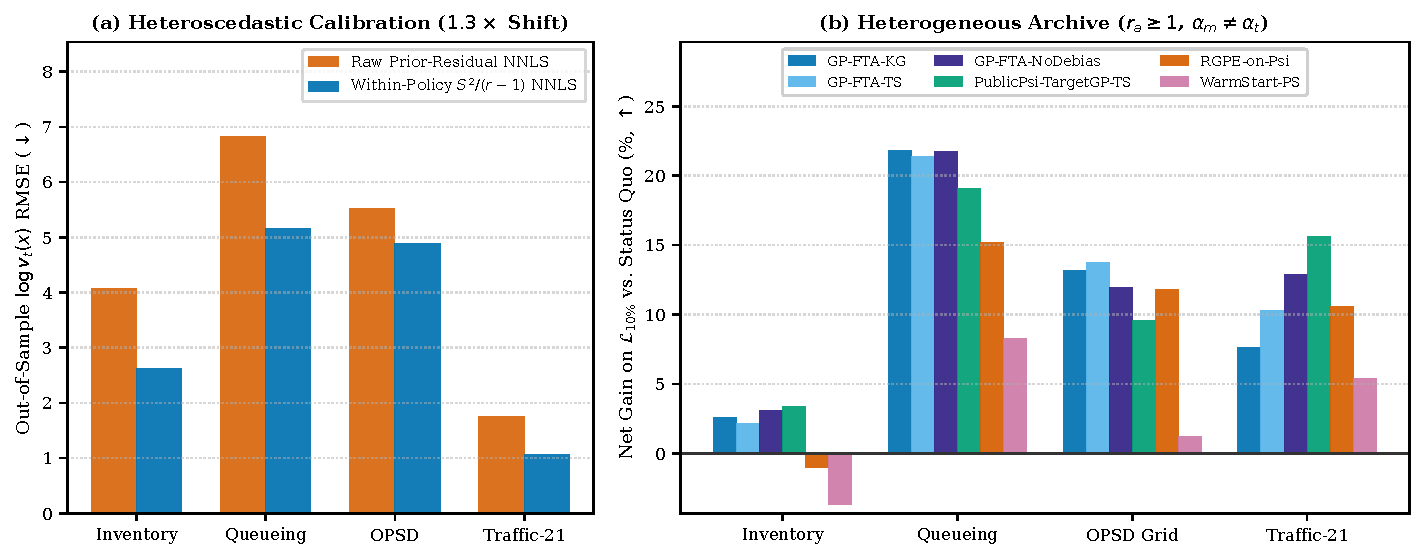
\includegraphics[width=0.98\textwidth]{figures/fig3_diagnostics_and_messy.pdf}
  \caption{(a) Out-of-sample heteroscedastic log-variance RMSE under $1.3\times$ target shift ($r=4$ replications), comparing raw prior-residual NNLS against shift-invariant within-policy $S^2/(r-1)$ NNLS. (b) Mean net gain on $\calL_{10\%}$ relative to status quo across all four operational domains under heterogeneous enterprise source archives ($r_a \ge 1$, $\alpha_m \neq \alpha_t$), including both \texttt{PublicPsi-TargetGP-TS} and \texttt{GP-FTA-NoDebias}.}\label{fig:ec_diagnostics}
\end{figure}

Figure~\ref{fig:ec_diagnostics} and Tables~\ref{tab:messy_archive}--\ref{tab:amortization} report the out-of-sample heteroscedastic calibration diagnostic, the $2{,}108$-run heterogeneous enterprise archive suite (comparing \textbf{GP-FTA-KG}, \textbf{GP-FTA-TS}, \texttt{GP-FTA-NoDebias}, \texttt{PublicPsi-TargetGP-TS}, \texttt{RGPE-on-Psi}, and \texttt{WarmStart-PatternSearch} side by side), the calibrated and stress-test live \texttt{Ingolstadt21} SUMO experiments, and source-archive simulation-call amortization against both raw-policy \texttt{SCBO} and same-representation \texttt{PublicPsi-TargetGP-TS}.

\begin{table}[htbp]
\centering
\caption{Heterogeneous simulated source archives on the shared U3 target panel ($2{,}108$ runs). Logs combine single replications, unequal budgets, incomplete solver coverage, and heterogeneous historical risk tolerances. Two-sided $p$ values compare status-quo loss with frozen GP-FTA-KG and are unadjusted. Online wall time is for $N=60$.}\label{tab:messy_archive}
\scriptsize
\resizebox{\textwidth}{!}{%
\begin{tabular}{llcccccc}
\toprule
\textbf{Family} & \textbf{Method} & \textbf{$N=15$ $\mathcal{L}_{\mathrm{SQ}}$} & \textbf{$N=60$ $\mathcal{L}_{\mathrm{SQ}}$} & \textbf{$N=60$ $\mathcal{L}_{10\%}$} & \textbf{$N=60$ Cert.\%} & \textbf{Two-Sided $p$ ($N=60$)} & \textbf{Online Wall (s)} \\
\midrule
\multirow{9}{*}{Inventory} & \textbf{GP-FTA-KG} & $1.941$ & $1.910$ & $1.910$ & 100.0\% & --- & 41.6 \\
 & \textbf{GP-FTA-TS} & $1.937$ & $1.914$ & $1.920$ & 96.9\% & $0.669$ & 10.0 \\
 & \texttt{GP-FTA-NoDebias} & $1.947$ & $1.901$ & $1.901$ & 100.0\% & $0.632$ & 44.2 \\
 & \texttt{RGPE-on-Psi} & $1.932$ & $1.926$ & $1.983$ & 71.9\% & $0.231$ & 12.4 \\
 & \texttt{WarmStart-PatternSearch} & $1.949$ & $1.943$ & $2.036$ & 53.1\% & $0.016$ & 0.3 \\
 & \texttt{PublicPsi-TargetGP-TS} & $\mathbf{1.909}$ & $\mathbf{1.883}$ & $\mathbf{1.895}$ & 93.8\% & $0.0004$ & 7.9 \\
 & \texttt{RGPE} & $1.963$ & $1.976$ & $1.989$ & 93.8\% & $0.002$ & 72.6 \\
 & \texttt{HyperBO-EB} & $1.974$ & $1.987$ & $1.987$ & 100.0\% & $0.0008$ & 2.1 \\
 & \texttt{STOP} & $1.996$ & $1.996$ & $1.996$ & 100.0\% & $0.003$ & 0.1 \\
\midrule
\multirow{9}{*}{Queueing} & \textbf{GP-FTA-KG} & $2.647$ & $\mathbf{2.518}$ & $\mathbf{2.518}$ & 100.0\% & --- & 44.5 \\
 & \textbf{GP-FTA-TS} & $2.627$ & $2.527$ & $2.527$ & 100.0\% & $0.375$ & 8.8 \\
 & \texttt{GP-FTA-NoDebias} & $\mathbf{2.584}$ & $2.519$ & $2.519$ & 100.0\% & $1.000$ & 44.9 \\
 & \texttt{RGPE-on-Psi} & $2.715$ & $2.688$ & $2.727$ & 87.5\% & $<10^{-4}$ & 10.5 \\
 & \texttt{WarmStart-PatternSearch} & $2.775$ & $2.864$ & $2.955$ & 71.9\% & $<10^{-4}$ & 0.4 \\
 & \texttt{PublicPsi-TargetGP-TS} & $2.704$ & $2.596$ & $2.607$ & 96.9\% & $0.003$ & 6.8 \\
 & \texttt{RGPE} & $3.047$ & $3.012$ & $3.042$ & 90.6\% & $<10^{-4}$ & 53.5 \\
 & \texttt{HyperBO-EB} & $3.056$ & $3.069$ & $3.085$ & 93.8\% & $<10^{-4}$ & 2.8 \\
 & \texttt{STOP} & $2.864$ & $2.864$ & $2.864$ & 100.0\% & $<10^{-4}$ & 0.1 \\
\midrule
\multirow{9}{*}{OPSD Grid} & \textbf{GP-FTA-KG} & $0.0606$ & $0.0568$ & $0.0572$ & 92.9\% & --- & 49.1 \\
 & \textbf{GP-FTA-TS} & $0.0582$ & $0.0566$ & $\mathbf{0.0570}$ & 92.9\% & $0.855$ & 11.1 \\
 & \texttt{GP-FTA-NoDebias} & $0.0589$ & $0.0569$ & $0.0573$ & 92.9\% & $0.903$ & 46.5 \\
 & \texttt{RGPE-on-Psi} & $\mathbf{0.0574}$ & $\mathbf{0.0562}$ & $0.0588$ & 64.3\% & $0.715$ & 13.6 \\
 & \texttt{WarmStart-PatternSearch} & $0.0609$ & $0.0614$ & $0.0635$ & 64.3\% & $0.004$ & 2.0 \\
 & \texttt{PublicPsi-TargetGP-TS} & $0.0607$ & $0.0583$ & $0.0590$ & 85.7\% & $0.358$ & 9.0 \\
 & \texttt{RGPE} & $0.0619$ & $0.0641$ & $0.0643$ & 96.4\% & $0.002$ & 173.9 \\
 & \texttt{HyperBO-EB} & $0.0607$ & $0.0618$ & $0.0626$ & 85.7\% & $0.005$ & 6.1 \\
 & \texttt{STOP} & $0.0639$ & $0.0639$ & $0.0639$ & 100.0\% & $0.0009$ & 0.4 \\
\midrule
\multirow{9}{*}{Traffic-21} & \textbf{GP-FTA-KG} & $1.102$ & $1.082$ & $1.110$ & 78.1\% & --- & 76.4 \\
 & \textbf{GP-FTA-TS} & $1.088$ & $1.061$ & $1.078$ & 87.5\% & $0.135$ & 37.4 \\
 & \texttt{GP-FTA-NoDebias} & $1.088$ & $1.034$ & $1.043$ & 93.8\% & $0.003$ & 78.2 \\
 & \texttt{RGPE-on-Psi} & $1.090$ & $1.055$ & $1.072$ & 87.5\% & $0.252$ & 45.3 \\
 & \texttt{WarmStart-PatternSearch} & $1.106$ & $1.096$ & $1.135$ & 68.8\% & $0.241$ & 2.1 \\
 & \texttt{PublicPsi-TargetGP-TS} & $\mathbf{1.050}$ & $\mathbf{1.007}$ & $\mathbf{1.007}$ & 100.0\% & $0.001$ & 34.3 \\
 & \texttt{RGPE} & $1.112$ & $1.094$ & $1.126$ & 75.0\% & $0.188$ & 13.1 \\
 & \texttt{HyperBO-EB} & $1.138$ & $1.137$ & $1.202$ & 46.9\% & $0.005$ & 2.7 \\
 & \texttt{STOP} & $1.088$ & $1.088$ & $1.113$ & 81.2\% & $0.524$ & 0.4 \\
\bottomrule
\end{tabular}%
}
\end{table}
\begin{table}[htbp]
\centering
\caption{Microscopic \texttt{Ingolstadt21} SUMO evaluation ($N=15$). The calibrated U3 panel has eight threshold and weight configurations of one network and route, with two simulation streams per configuration. The 40 uncalibrated stress runs were retained from the earlier experiment.}\label{tab:live_sumo}
\scriptsize
\setlength{\tabcolsep}{4.6pt}
\begin{tabular}{llccccc}
\toprule
\textbf{Regime} & \textbf{Method} & \textbf{Status-Quo Loss} & \textbf{Challenger $J_t^{\ddagger}$} & \textbf{Cert./runs} & \textbf{S/A/U$^*$} & \textbf{Actual Calls} \\
\midrule
\multirow{9}{*}{Calibrated ($144$ runs)} & \textbf{GP-FTA-KG} & $\mathbf{0.9439} \pm 0.0181$ & $0.9340$ & 8/16 & 3/5/0 & 344.8 \\
 & \texttt{PublicPsi-TargetGP-TS} & $0.9696 \pm 0.0088$ & $0.9661$ & 5/16 & 3/2/0 & 387.8 \\
 & \textbf{GP-FTA-TS} & $0.9737 \pm 0.0090$ & $0.9647$ & 5/16 & 1/4/0 & 362.2 \\
 & \texttt{SCBO-on-Psi} & $0.9829 \pm 0.0050$ & $0.9735$ & 3/16 & 2/1/0 & 379.8 \\
 & \texttt{RGPE-on-Psi} & $0.9850 \pm 0.0058$ & $1.0247$ & 2/16 & 0/2/0 & 396.5 \\
 & \texttt{WarmStart-PatternSearch} & $0.9871 \pm 0.0037$ & $0.9898$ & 3/16 & 1/2/0 & 379.8 \\
 & \texttt{RGPE} & $0.9941 \pm 0.0012$ & $1.0164$ & 0/16 & --- & 422.0 \\
 & \texttt{SCBO} & $0.9941 \pm 0.0012$ & $0.9909$ & 0/16 & --- & 422.0 \\
 & \texttt{STOP} & $0.9941 \pm 0.0012$ & $0.9878$ & 0/16 & --- & 392.0 \\
\midrule
\multirow{5}{*}{Stress Test ($40$ runs)} & \texttt{TLS-OLH-KG} (Legacy) & $0.9876$ & $0.9642$ & 0/8 & --- & 422.0 \\
 & \texttt{SCBO} & $0.9876$ & $0.9826$ & 0/8 & --- & 422.0 \\
 & \texttt{RGPE} & $0.9876$ & $0.9888$ & 0/8 & --- & 422.0 \\
 & \texttt{Target-SPSA} & $0.9876$ & $0.9645$ & 0/8 & --- & 422.0 \\
 & \texttt{STOP} & $0.9876$ & $0.9876$ & 0/8 & --- & 392.0 \\
\bottomrule
\end{tabular}
\par\smallskip\parbox{\textwidth}{\scriptsize $^*$S/A/U counts certified deployments classified as confidently safe, boundary-ambiguous, or confidently unsafe by an independent audit. A dash indicates no audited deployment. $^{\ddagger}$Calibrated runs use the frozen primary. Stress runs use the saved uncertified candidate.}
\end{table}
\begin{table}[htbp]
\centering
\caption{Source-archive simulation-call amortization ($B_{\mathrm{src}}=1{,}428$ calls per family) comparing low-budget \textbf{GP-FTA-KG} ($N=15$) against both raw-policy \texttt{SCBO} ($N=60$) and same-representation \texttt{PublicPsi-TargetGP-TS} ($N=60$). Full-cost break-even $M_{\mathrm{break}}^{\mathrm{full}}$ is reported only when \textbf{GP-FTA-KG} ($N=15$) attains equal or lower mean $\mathcal{L}_{\mathrm{SQ}}$ than the $N=60$ cold-start comparator (`Not dom.' indicates the $N=60$ cold-start representation control achieves lower loss).}\label{tab:amortization}
\scriptsize
\resizebox{\textwidth}{!}{%
\begin{tabular}{llcccccc}
\toprule
\textbf{Comparator ($N=60$)} & \textbf{Family} & \textbf{GP-FTA ($N\!=\!15$)} & \textbf{Cold ($N\!=\!60$)} & \textbf{$B_{\mathrm{FTA},15}$ / $B_{\mathrm{cold},60}$} & \textbf{Call Saving $\Delta B$ [95\% CI]} & \textbf{$M_{\mathrm{break}}^{\mathrm{sunk}}$} & \textbf{$M_{\mathrm{break}}^{\mathrm{full}}$ (95\% UB)} \\
\midrule
\multirow{4}{*}{\texttt{SCBO}} & Inventory & $1.927$ & $1.960$ & 238.8 / 350.2 & $+111.5$ $[+54.2, +168.8]$ & $1$ & $\mathbf{13}$ ($\le 27$) \\
 & Queueing & $2.535$ & $3.052$ & 254.4 / 312.4 & $+58.0$ $[+16.0, +100.0]$ & $1$ & $\mathbf{25}$ ($\le 90$) \\
 & OPSD Grid & $0.0587$ & $0.0610$ & 260.3 / 406.4 & $+146.1$ $[+106.2, +186.1]$ & $1$ & $\mathbf{10}$ ($\le 14$) \\
 & Traffic-21 & $1.108$ & $1.145$ & 285.4 / 426.8 & $+141.4$ $[+103.2, +179.5]$ & $1$ & $\mathbf{11}$ ($\le 14$) \\
\midrule
\multirow{4}{*}{\texttt{PublicPsi-TargetGP-TS}} & Inventory & $1.927$ & $1.883$ & 238.8 / 390.2 & $+151.5$ $[+111.4, +191.6]$ & Not dom. & Not dom. \\
 & Queueing & $2.535$ & $2.596$ & 254.4 / 385.1 & $+130.8$ $[+97.0, +164.5]$ & $1$ & $\mathbf{11}$ ($\le 15$) \\
 & OPSD Grid & $0.0587$ & $0.0583$ & 260.3 / 416.0 & $+155.7$ $[+121.8, +189.7]$ & Not dom. & Not dom. \\
 & Traffic-21 & $1.108$ & $1.007$ & 285.4 / 372.4 & $+87.0$ $[+40.0, +134.0]$ & Not dom. & Not dom. \\
\bottomrule
\end{tabular}%
}
\end{table}

